\pagebreak
\newsection{Architettura}
All'interno della seguente sezione verrà descritta l'architettura dell'intero sistema.
Per la realizzazione dell'architettura del plugin il team ha deciso di adottare uno stile architetturale a layer.\\
I principali layer che sono stati individuti nel corso dello sviluppo dell'applicazione sono i seguenti:
\begin{itemize}
	\item{\textbf{Presentation layer}: si occupa di gestire la componente grafica del panel;}
	\item{\textbf{Persistence layer}: si occupa di mantenere la struttura della rete;}
	\item{\textbf{Buisness layer}: incorpora tutta la logica relativa all’intero processo di ricalcolo delle probabilità;}
	\item{\textbf{Database layer}: composto dall’insieme di tutti i database esterni forniti dall’utente per il reperimento delle informazioni.}
\end{itemize}
\begin{figure} [H]
	\centering
	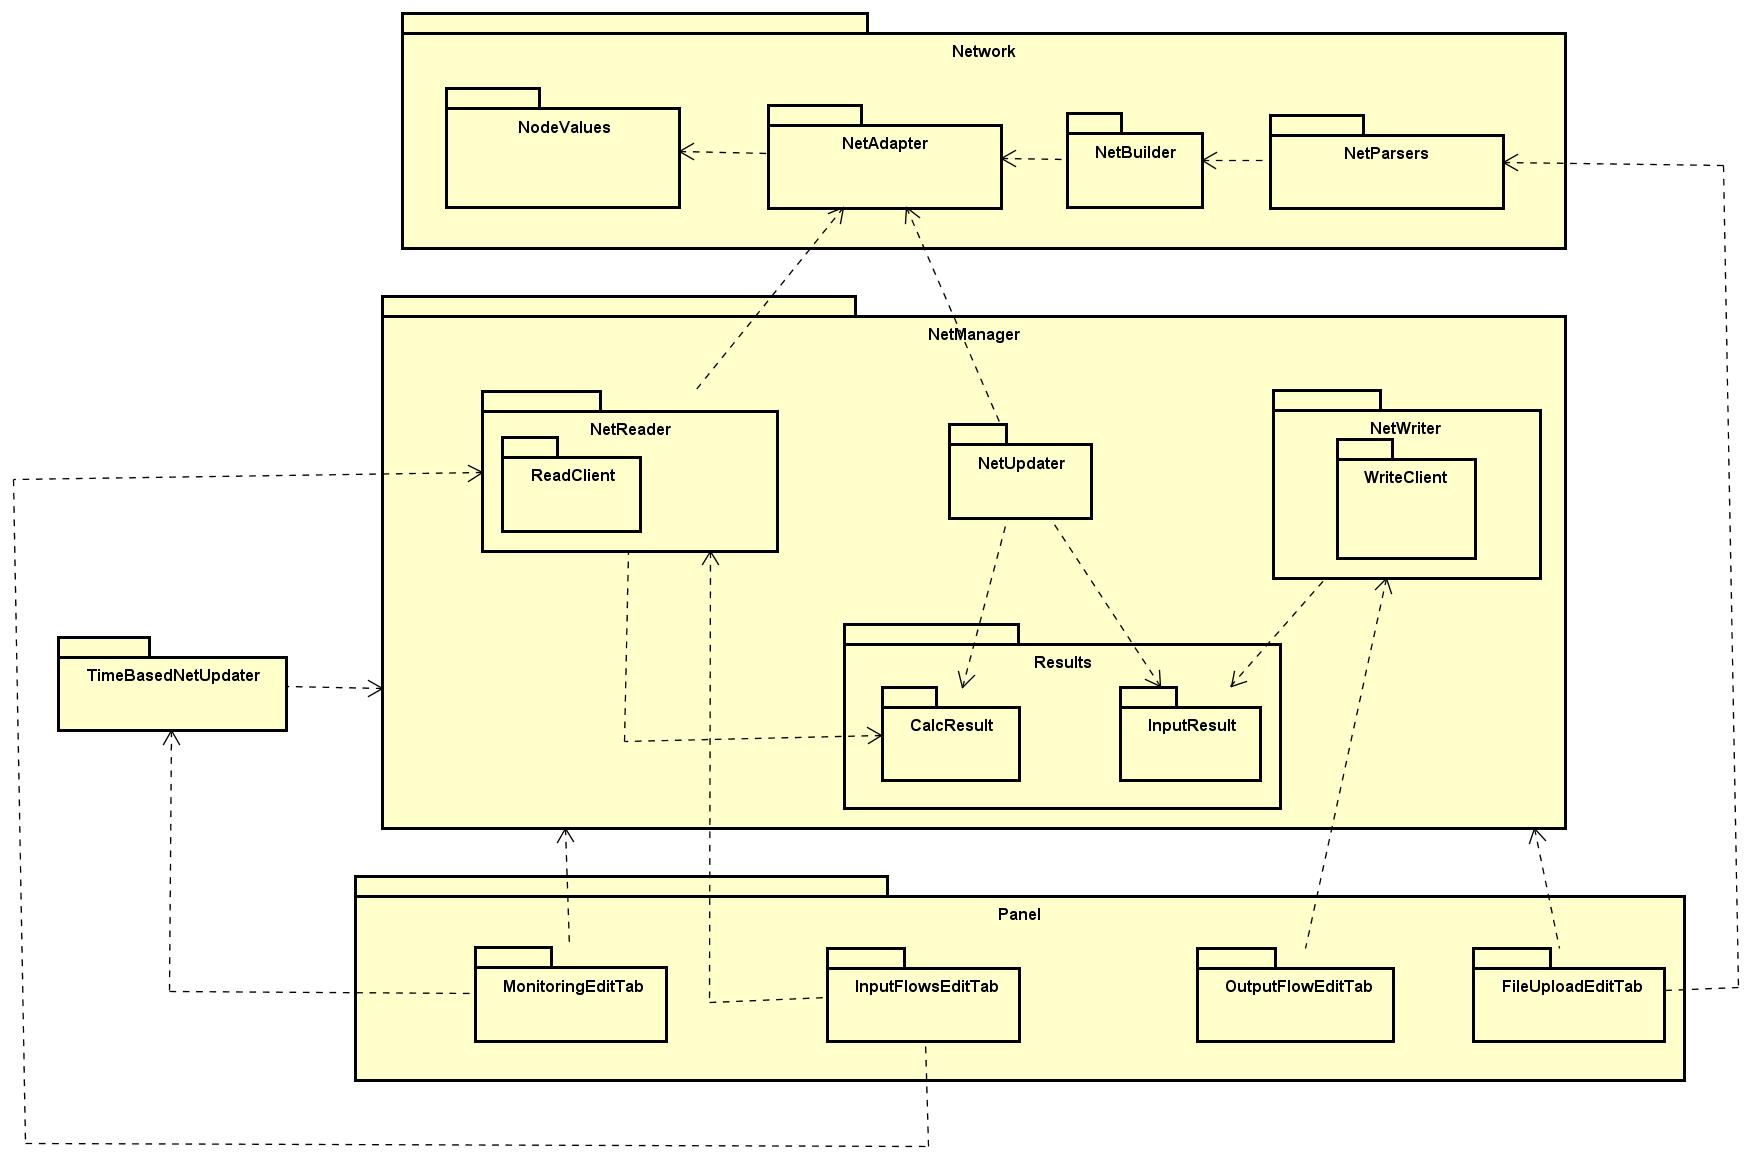
\includegraphics[scale=0.25]{Img/Diagramma_Package}
	\caption{Diagramma dei package}\label{}
\end{figure}
\begin{figure} [H]
	\centering
	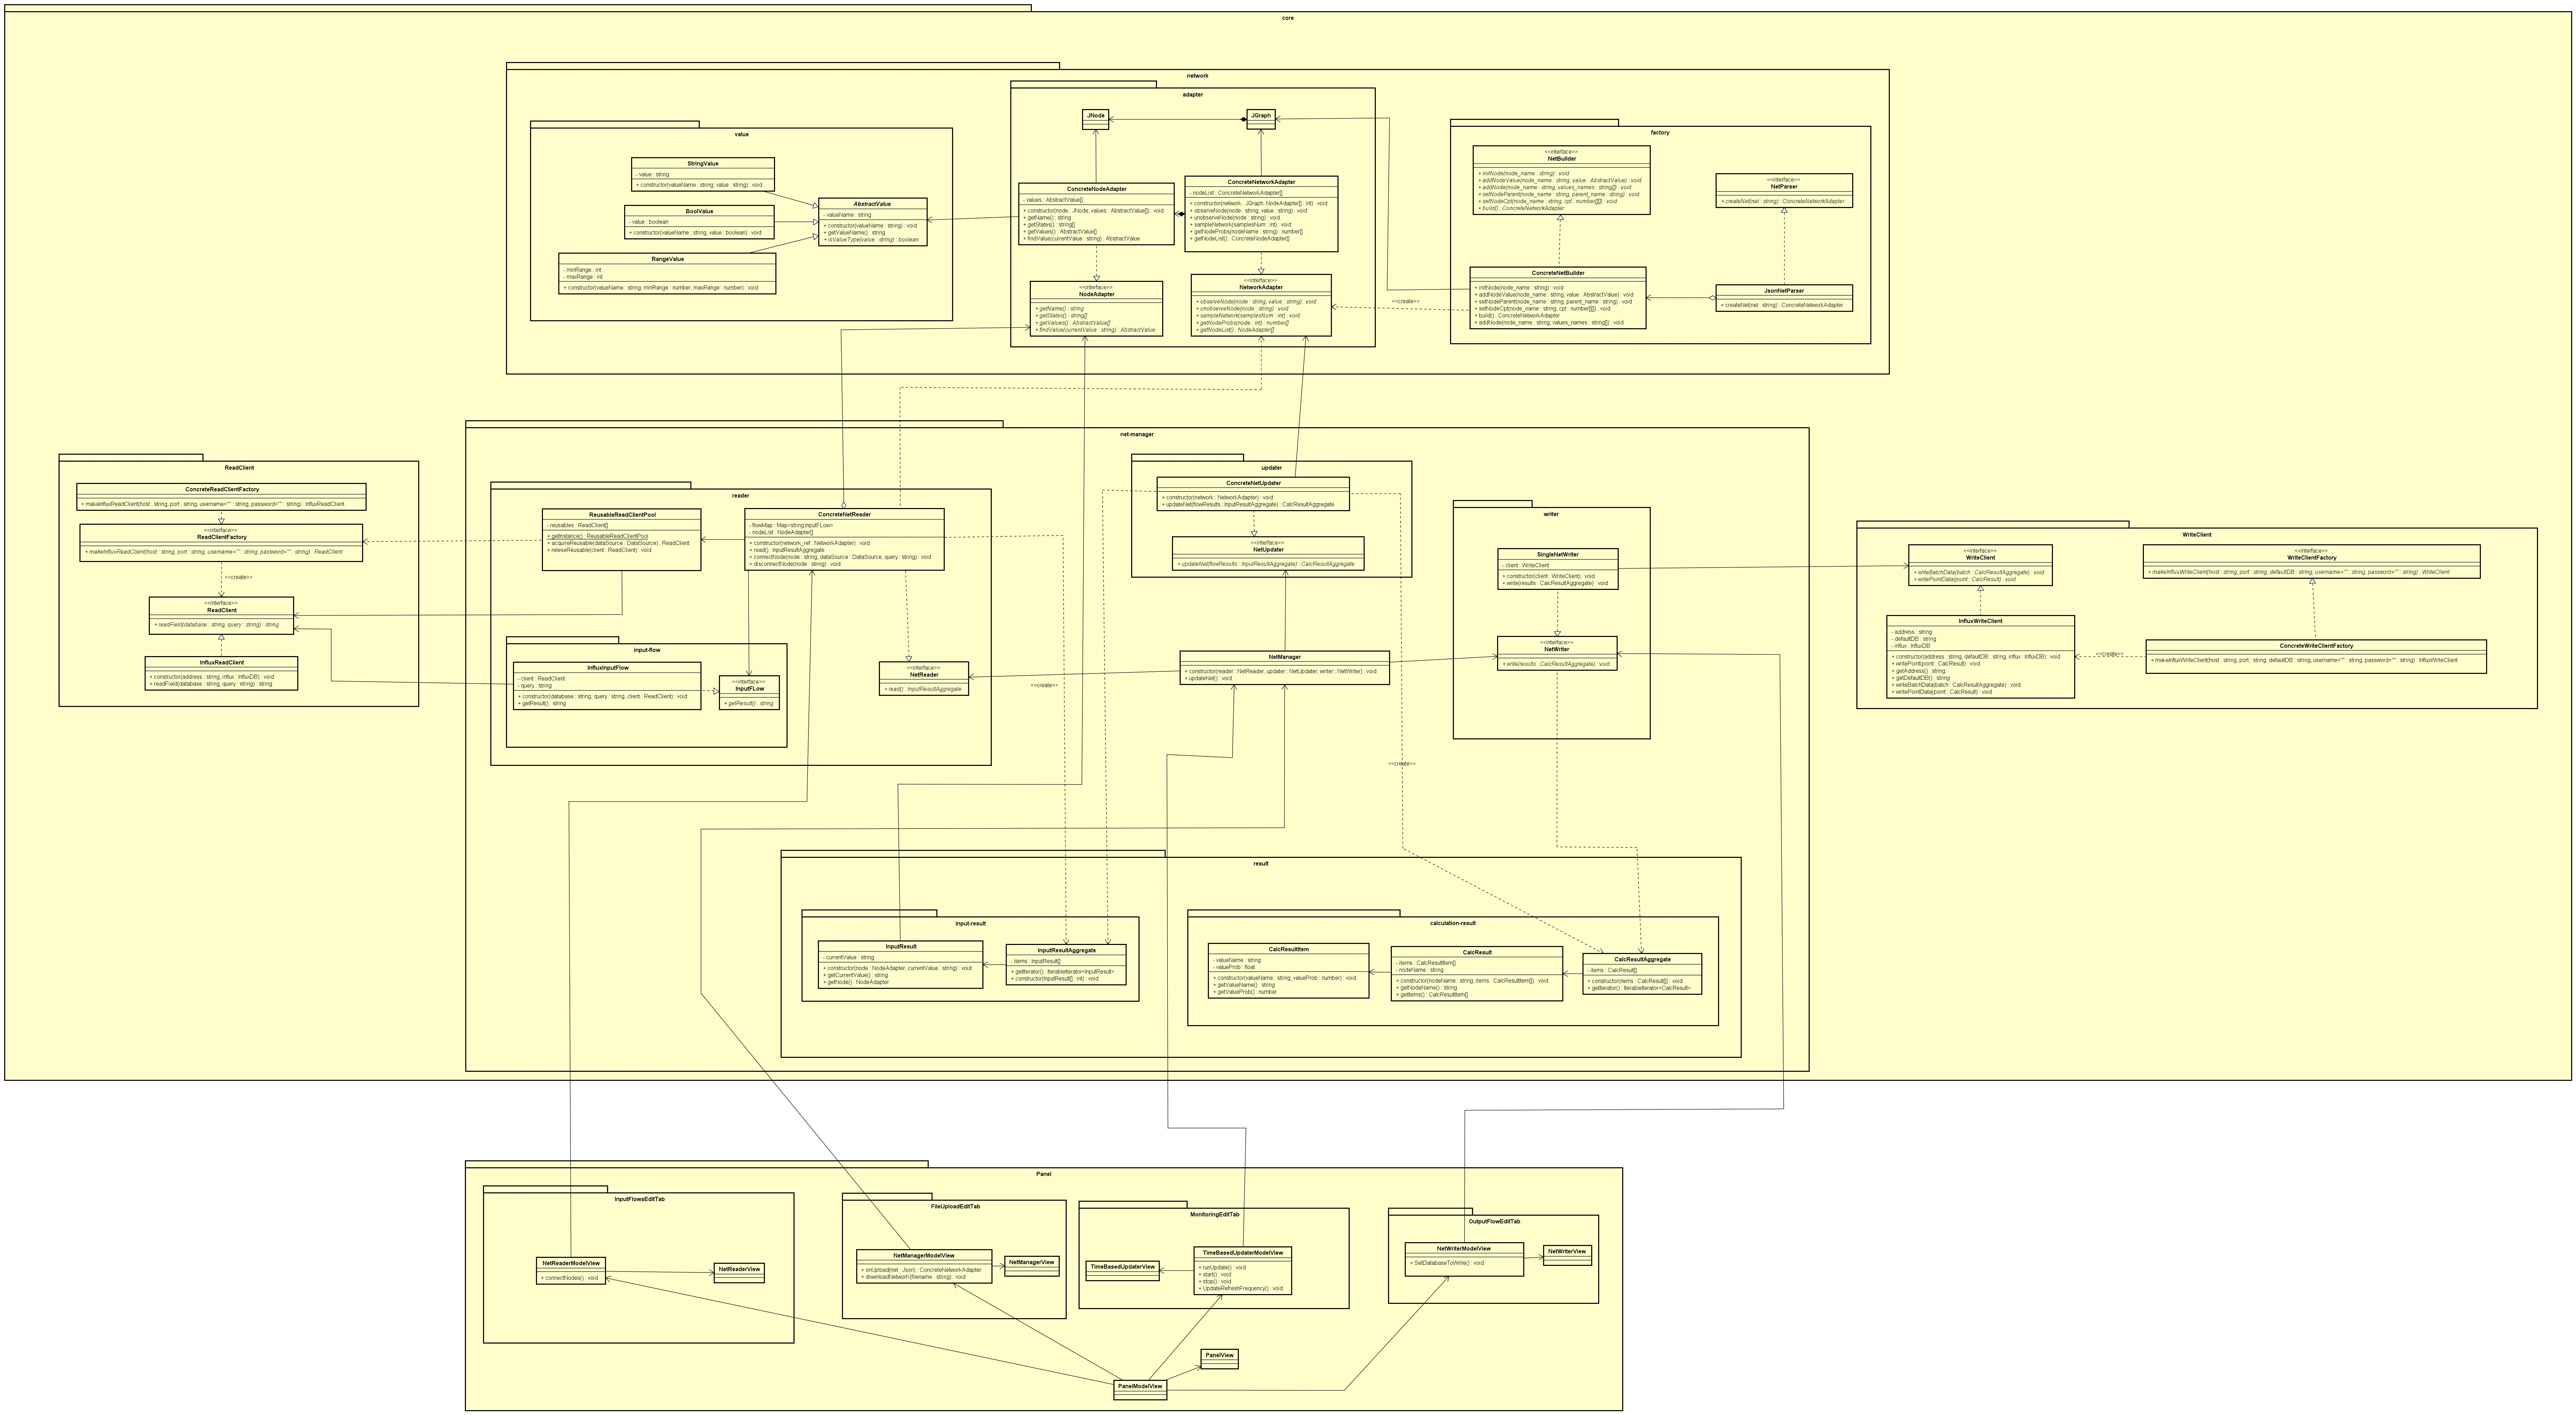
\includegraphics[scale=0.05]{Img/Diagramma_Classi}
	\caption{Diagramma delle classi complessivo}\label{}
\end{figure}
Analizziamo ora più in dettaglio ciascuno dei layer precedentemente descritti.
\subsection{Persistence Layer}
L'intera nostra applicazione è basata sulla libreria Javascript JSBayes consigliata dal proponente, la quale permette di mantenere l'intera struttura della rete ed esegue su di essa il calcolo delle probabilità di ogni stato associato ad ogni nodo della rete.
Questa libreria tuttavia presenta non pochi problemi, tra i quali una pressochè totale assenza della gestione degli errori, una difficile interazione con altri oggetti, ed una scarsa estendibilità.
Il persistence layer è composto principalmente da un insieme di classi che permettono di ovviare ai problemi precedentemente descritti.
\subsubsection{NetworkAdapter}
La classe NetworkAdapter ha il compito di schermare tutte le operazioni non sicure di JSBayes, cioè quelle che vanno a modificare la struttura della rete rischiando quindi di minare la potenziale integrità dei dati.
Essa espone solamente i metodi necessari per effettuare il ricalcolo delle probabilità e che quindi non modificano in alcun modo lo stato.
\begin{figure} [H]
	\centering

	\caption{Diagramma UML NetworkAdapter}\label{}
\end{figure}
\subsubsection{NodeAdapter}
Per lo sviluppo delle funzionalità del plugin il team ha avuto la necessità di aggiungere informazioni ai singoli nodi della rete bayesiana memorizzata da JSBayes.
Estendere dalle classi offerte dalla libreria era impensabile a causa dei molteplici problemi descritti all'inizio di questa sezione. Per questo motivo abbiamo deciso di realizzare un adapter anche per i singoli nodi di JSBayes ed includere all'interno di questi tutte le informazioni aggiuntive necessarie, come gli AbstractValue che verranno descritti in dettaglio all'interno della sezione seguente.
\begin{figure} [H]
	\centering
	
	\caption{Diagramma UML NodeAdapter}\label{}
\end{figure}
\subsubsection{AbstractValue}
Per poter determinare in quale stato il nodo si trova sulla base dei dati prelevati da una qualsiasi fonte dati, come un database, il semplice nome che JSBayes associa ad ogni stato non era sufficiente.\\
Il compito degli AbstractValue è proprio quello di colmare questa lacuna.
Invocando su un oggetto AbstractValue il metodo
\begin{ttfamily}
	isValueType(value:string):bool
\end{ttfamily}
e passandogli come parametro il risultato di una lettura da una qualsiasi fonte dati l'AbstractValue ritorna un boolean indicando all'invocatore se lo stato associato è attualmente vero o meno.\\
Il team ha realizzato solamente tre implementazioni concrete di abstract value, rispettivamente RangeValue, StringValue e BoolValue, tuttavia è possibile realizzare altre implementazioni semplicemente estendendo dall'interfaccia AbstractValue.
\begin{figure} [H]
	\centering
	
	\caption{Diagramma UML AbstractValue}\label{}
\end{figure}
\subsubsection{NetBuilder}
Per garantire l'integrità dei dati abbiamo deciso di esternare il processo di creazione della rete JSBayes all'interno di un builder esterno il quale ha il compito di effettuare tutti i controlli necessari e ritornare un riferimento ad un NetworkAdapter solo al termine dell'intero processo di creazione invocando il metodo
\begin{ttfamily}
	build()
\end{ttfamily}.
\begin{figure} [H]
	\centering
	
	\caption{Diagramma UML NetBuilder}\label{}
\end{figure}
\subsubsection{NetParser}
Il NetParser ha il compito di realizzare un NetAdapter, sfruttando le funzionalità esposte dal NetBuilder, a partire dal contenuto di un file di testo.
Il team fino ad ora ha realizzato un unica implementazione, quella relativa a file di tipo JSON in quanto era l'unico formato richiesto dal proponente.
Nel caso in cui un giorno fosse necessario utilizzare formati differenti è sarà sufficiente realizzare una differente implementazione dell'interfaccia NetParser.
\begin{figure} [H]
	\centering
	
	\caption{Diagramma UML NetParser}\label{}
\end{figure}
\subsection{Buisness Layer}
Il buisness layer ingloba all'interno di esso tutta la logica relativa al processo di calcolo delle probabilità.
Dopo un attenta analisi del problema il team è riuscito a scomporre il suddetto processo in 3 macro-fasi principali:
\begin{itemize}
	\item La lettura dei dati dai database associati ai nodi delle rete;
	\item Il processo di calcolo delle probabilità vero e proprio partendo dai dati letti precedentemente.
	\item La scrittura delle probabilitá appena calcolate su un database che l'utente poi potrá utilizzare per fare la visualizzazione dei dati su grafana
\end{itemize}
Ci è sembrato dunque abbastanza naturale modellare l'architettura del buisness layer in tre oggetti distinti ognuno dei quali si occupa di gestire una specifica fase del processo dall'inizio alla fine.
Analizziamo ora più in dettaglio gli oggetti precedentemente citati.
\subsubsection{NetReader}
Il NetReader è collegato ad un ReadClient, di cui parleremo successivamente all'interno della sezione dedicata al database layer. NetReader è responsabile di collegare un nodo ad un flusso di dati e di richiedere a ReadClient di interrogare il database per ottenere i dati necessari.\\
Per non dover istanziare più client di lettura per la stessa sorgente dati o database, abbiamo implementato una Object Pool per i client di lettura: quando si connette un nodo ad un flusso di dati, se il client richiesto esiste viene estratto dal pool, altrimenti viene creato ad-hoc.
\begin{figure} [H]
	\centering
	
	\caption{Diagramma UML NetReader}\label{}
\end{figure}
\subsubsection{NetUpdater}
NetUpdater ha il compito di effettuare il ricalcolo utilizzando i dati letti da NetReader e le funzionalità esposte dal NetworkAdapter.
\begin{figure} [H]
	\centering
	
	\caption{Diagramma UML NetUpdater}\label{}
\end{figure}
\subsubsection{NetWriter}
\begin{figure} [H]
	\centering
	
	\caption{Diagramma UML NetWriter}\label{}
\end{figure}
\subsubsection{NetManager}
Il NetManager non è altro che un facade il quale ha un riferimento ad un istanza di NetReader, NetUpdater e NetWriter ciascuna. Esso ha il compito di coordinare l'intero processo di calcolo delle probabilità invocando sequenzialmente le operazioni giuste nell'ordine corretto.
\begin{figure} [H]
	\centering
	
	\caption{Diagramma UML NetManager}\label{}
\end{figure}
\subsubsection{Results}

\subsection{Database Layer}
\subsection{Presentation Layer}
\pagebreak